\documentclass[../PianoDiQualifica.tex]{subfiles}
\begin{document}
	\section{Design pattern utilizzati}
		\subsection{Architetturali}
			\subsubsection{MVC}
					\begin{figure}[H] \label{fig:MVC}
					\centering
					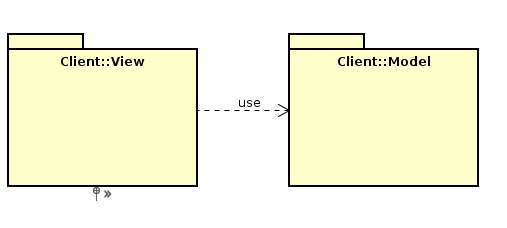
\includegraphics[scale=0.8]{Immagini/MVC.png}
					\caption{Esempio pattern MVC}
				\end{figure}
				\paragraph{Scopo\\}
				Pattern architetturale per la progettazione e strutturazione modulare di applicazioni software interattive.
				Consente di separare e disaccoppiare i componenti software che implementano il modello delle informazioni, dai
				componenti che implementano la logica di presentazione e la logica di controllo che gestiscono tali informazioni. 
				\paragraph{Problema\\}
				L'applicazione deve avere una natura modulare e basata sulle responsabilità, al fine di ottenere una vera e propria applicazione component - based. Questo è conveniente per poter più facilmente gestire la manutenzione dell'applicazione. \\
				L'applicazione deve separare i componenti software che implementano il modello delle funzionalità di business, dai componenti che implementano la logica di presentazione e di controllo che utilizzano tali funzionalità.
				\paragraph{Struttura\\}			
				\begin{itemize}
					\item Model : Definisce le regole di business per l’interazione con i dati, esponendo alla View ed al Controller rispettivamente le funzionalità per l’accesso e l’aggiornamento.
					Ha la responsabilità di notificare ai componenti della View eventuali aggiornamenti verificatisi in seguito a richieste del Controller, al fine di permettere alle View di presentare dati sempre aggiornati;
					\item View : Gestisce la logica di presentazione dei dati;
					\item Controller : implementa la logica di controllo dell’applicazione. Nella nostra particolare architettura, questa componente non è indipendente, ma bensì implementata dalla View, come in accordo con il framework utilizzato, ovvero Backbone.
				\end{itemize}			
				\paragraph{Utilizzo nel progetto\\}
				Pattern architetturale utilizzato nella componente di front-end, ovvero SWEDesigner::Client. Tale pattern è stato adattato per rispecchiare il modello architetturale previsto da Backbone, il framework utilizzato per sviluppare la parte di front-end.
				
			\subsubsection{Data Access Object}
			\begin{figure}[H] \label{fig:DAO}
				\centering
				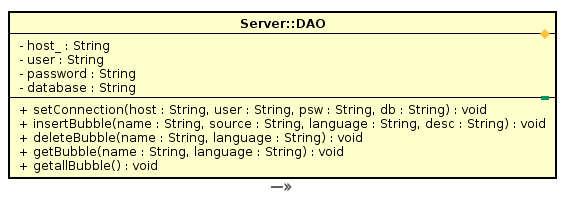
\includegraphics[scale=0.8]{Immagini/DAO.png}
				\caption{Esempio pattern DAO}
			\end{figure}
			\paragraph{Scopo\\}
			 Pattern architetturale per la gestione della persistenza: si tratta fondamentalmente di una classe con relativi metodi che rappresenta un'entità tabellare di un RDBMS, usata per stratificare e isolare l'accesso ad una tabella tramite query (poste all'interno dei metodi della classe) ovvero al data layer da parte della business logic creando un maggiore livello di astrazione ed una più facile manutenibilità.
			\paragraph{Problema\\}
			Necessità di separare le logiche di business da quelle di accesso ai dati; incapsulare l'accesso ai dati persistenti in un oggetto e fornire un'interfaccia 
			per la manipolazione di tali dati.
			\paragraph{Struttura\\}
			Composto da un'unica componente, DAO, che espone le funzionalità per accedere ai dati persistenti.			
			\paragraph{Utilizzo nel progetto\\}
			Utilizzato nella parte di back-end, per gestire la persistenza e gestione delle bubble.
			
		\subsection{Strutturali}
%			\subsubsection{Decorator}
%				\begin{figure}[H] \label{fig:Decorator}
%					\centering
%					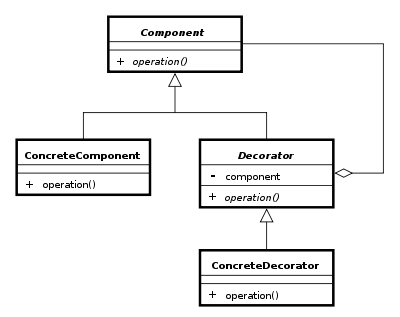
\includegraphics[scale=0.8]{Immagini/DecoratorEx.png}
%					\caption{Esempio pattern Decorator}
%				\end{figure}
%				\paragraph{Scopo\\}
%					Aggiungere responsabilità ad un oggetto dinamicamente.
%				\paragraph{Problema\\}
%					Si vuole aggiungere comportamento o stato ai singoli oggetti durante l'esecuzione
%					e l'ereditarietà non è fattibile perché è statico e si applica ad un'intera classe.
%				\paragraph{Struttura\\}
%					Sono individuabili le seguenti componenti principali:
%					\begin{itemize}
%						\item Component: interfaccia degli oggetti che dovranno essere estesi;
%						\item ConcreteComponent: l'oggetto da estendere;
%						\item Decorator: ha un riferimento all'oggetto Component e
%						definisce un'interfaccia conforme a quella Component;
%						\item ConcreteDecorator: aggiunge funzionalità al Component.
%					\end{itemize}
%				\paragraph{Utilizzo nel progetto\\}
%					% DA AGGIUNGERE (TO DO)
			\subsubsection{Facade}
				\begin{figure}[H] \label{fig:Facade}
					\centering
					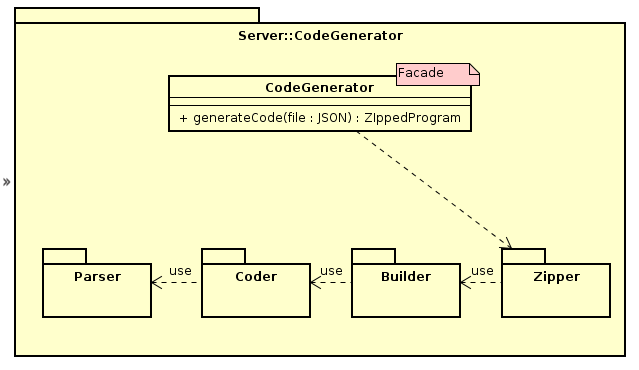
\includegraphics[scale=0.8]{Immagini/FacadeEx.png}
					\caption{Esempio pattern Facade}
				\end{figure}
				\paragraph{Scopo\\}
					Fornire un'interfaccia unificata per l'accesso ad uno o più sottosistemi complessi
					nascondendone la complessità all'esterno. Strutturare un sistema in sottosistemi aiuta a ridurre la complessità; un obiettivo comune è minimizzare la comunicazione tra questi sottosistemi: una soluzione è introdurre un oggetto Facade che fornisca una singola, semplificata interfaccia alle funzioni più generali di un sottosistema.
				\paragraph{Problema\\}
					I sottosistemi, man mano che evolvono, tendono a creare molte e piccole classi, al fine di aumentare la riusabilità e la facilità di personalizzazione, ma in questo modo diventano complesse da utilizzare e la maggior parte dei clients non necessitano di conoscere i dettagli del sottosistema; un Facade fornisce una semplice interfaccia, ma sufficiente alla maggior parte dei clients, di un sistema complesso.
				\paragraph{Struttura\\}
					La principale componente individuabile è la classe Facade che si interpone tra il
					sottosistema e l'esterno, ed associa ogni richiesta ad una classe del sottosistema,
					delegando la risposta.
					\begin{itemize}
						\item Facade : espone le funzionalità di cui necessitano la maggior parte dei client, nascondendo la complessità del sottosistema; Nella figura, tale componente è rappresentata dalla classe CodeGenerator, che espone la funzionalità di creazione del programma richiesto dal client;
						\item Sottosistema: Implementano le funzionalità del sottosistema; gestiscono le attività assegnate dal Facade e non hanno nessun riferimento ad esso. Nella figura, il sottosistema è composto dai moduli Parser, Coder,Builder e Zipper, i quali si occupano di implementare la funzionalità di generazione del programma.
					\end{itemize}
					
				\paragraph{Utilizzo nel progetto\\}
					Utilizzato, ad esempio, lato server nel CodeGenerator in cui la classe CodeGenerator funge da Facade e espone la funzionalità che permette la generazione del codice sorgente, senza dover interfacciarsi con i vari moduli che implementano tale funzionalità.
		\subsection{Creazionali}
			\subsubsection{Builder}
				\begin{figure}[H] \label{fig:Builder}
					\centering
					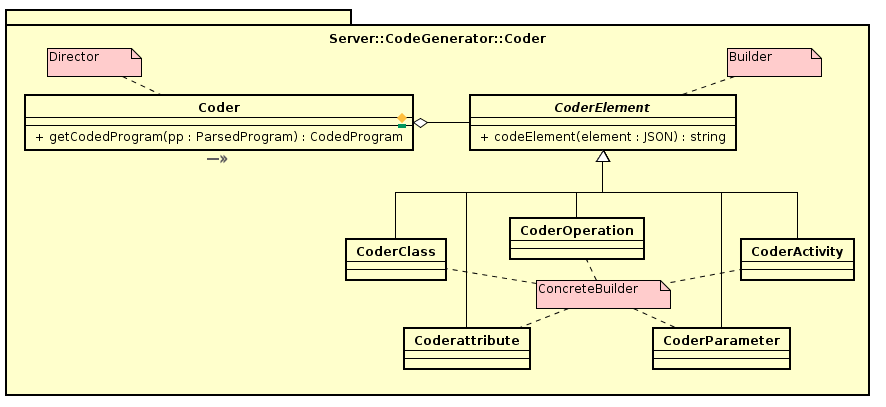
\includegraphics[scale=0.8]{Immagini/Builder.png}
					\caption{Esempio pattern Builder}
				\end{figure}
				\paragraph{Scopo\\}
					Separa la costruzione di un oggetto complesso dalla sua
					rappresentazione, in modo che lo stesso processo di costruzione
					consenta la creazione di diverse rappresentazioni.
				\paragraph{Problema\\}
					L'algoritmo di creazione di un oggetto complesso dovrebbe essere indipendente dalle parti che compongono l'oggetto e da come queste sono assemblate.
				\paragraph{Struttura\\}
				Il “Builder” pattern propone separare la “logica del processo di
				costruzione” dalla “costruzione stessa”. Per fare ciò si utilizza un oggetto
				Director, che determina la logica di costruzione del prodotto, e che invia
				le istruzioni necessarie ad un oggetto Builder, incaricato della sua
				realizzazione. Siccome i prodotti da realizzare sono di diversa natura, ci
				saranno Builder particolari per ogni tipo di prodotto, ma soltanto un unico
				Director, che nel processo di costruzione invocherà i metodi del Builder
				scelto secondo il tipo di prodotto desiderato (i Builder dovranno
				implementare un’interfaccia comune per consentire al Director di
				interagire con tutti questi). \\
					Sono individuabili quattro componenti principali:
					\begin{itemize}
						\item Director: Costruisce un oggetto utilizzando il builder (procedura). Nella figura, tale componente è rappresentata da Coder;
						\item Builder: Specifica l’interfaccia da utilizzare per assemblare il prodotto. Nella figura, tale componente è rappresentata da CoderElement;
						\item ConcreteBuilder: Costruisce e assembla le parti del
						prodotto. Tiene traccia dell’istanza costruita. Fornisce un’interfaccia per recuperare il prodotto finale. Nella figura, sono presenti diverse componenti di questo tipo: CoderClass, CoderOperation, CoderActivity, CoderAttribute, CoderParameter;
						\item Product: Prodotto da costruire. Nel nostro caso non si tratta di uno specifico oggetto, ma bensì della stringa che rappresenta il codice sorgente creato dalo specifico ConcreteBuilder.
					\end{itemize}
				\paragraph{Utilizzo nel progetto\\}
					Utilizzato, ad esempio, lato server nella componente Coder per costruire i vari elementi codificati di una classe.
		\subsection{Comportamentali}
% Observer da rivedere dopo aver progettato in dettaglio la view
			\subsubsection{Observer}
				\begin{figure}[H] \label{fig:Observer}
					\centering
					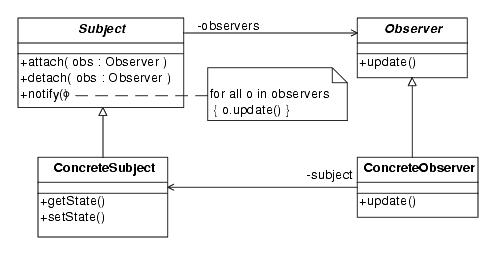
\includegraphics[scale=0.6]{Immagini/ObserverEx.png}
					\caption{Esempio pattern Observer}
				\end{figure}
				\paragraph{Scopo\\}
					Definire una dipendenza "1..n" fra oggetti, riflettendo le modifiche dell'oggetto
					sui suoi dipendenti. Consente la definizione di associazioni di dipendenza di molti oggetti verso di uno, in modo che se quest’ultimo cambia il suo stato, tutti gli altri sono notificati e aggiornati automaticamente.
				\paragraph{Problema\\}
					Il cambiamento si stato di un oggetto richiede la modifica dello stato di altri oggetti, senza conoscere quanti oggetti hanno effettivamente bisogno di cambiare il loro stato. \\
					Un oggetto deve avere la capacità di notificare altri oggetti senza fare assunzioni su chi questi oggetti siano; in altre parole, non si vuole che questi oggetti siano fortemente accoppiati.
				\paragraph{Struttura\\}
					Sono individuabili quattro componenti principali:
					\begin{itemize}
						\item ConcreteSubject: mantiene lo stato di un oggetto concreto, notificando
						gli osservatori concreti in caso di cambiamenti. Nella figura, tale componente è rappresentata da SWEDedigner::Client::Model::MainModel;
						\item ConcreteObserver: esplicita le azioni da eseguire qualora si verifichi un cambio di stato
						dell'oggetto osservato. Nella figura, tale componente è rappresentata da SWEDedigner::Client::View::MainView;
					\end{itemize}
				\paragraph{Utilizzo nel progetto\\}
					Utilizzato, ad esempio, lato client dalla View per osservare i cambiamenti del
					Model; la sua implementazione è fornita da Backbone.js.
			\subsubsection{Command}
				\begin{figure}[H] \label{fig:Command}
					\centering
					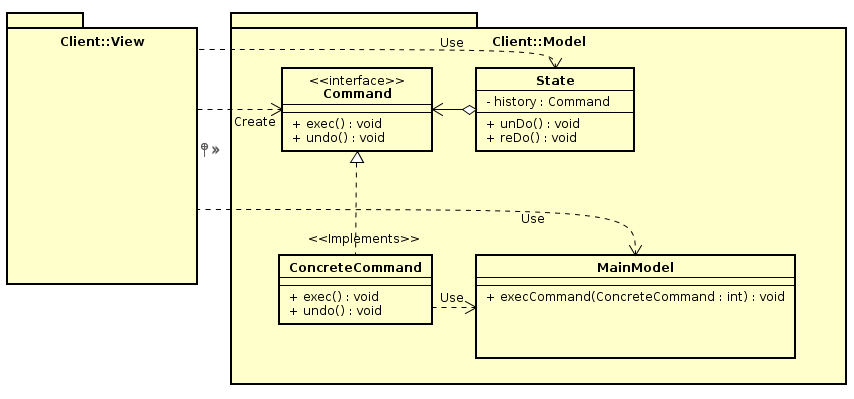
\includegraphics[scale=0.8]{Immagini/CommandEx.png}
					\caption{Esempio pattern Command}
				\end{figure}
				\paragraph{Scopo\\}
					Incapsulare il codice che effettua un'azione separandolo dall'oggetto che ne
					richiede l'esecuzione. Incapsula una richiesta all’interno di un oggetto, cosicché i client siano indipendenti dalle richieste; questo consente la parametrizzazione dei client con diverse tipologie di richieste, accodare o rintracciare le richieste, oppure supportare operazioni di undo.
				\paragraph{Problema\\}
					Necessità di gestire richieste di cui non si conoscono i particolari; ovvero le effettive operazioni che verranno richieste e/o i ricevitori di
					tali richieste. \\
					Necessità di fornire operazioni di undo.
				\paragraph{Struttura\\}
					Sono individuabili quattro componenti principali:
					\begin{itemize}
						\item Receiver: conosce l'effettiva implementazione dell'operazione/i associata con la gestione di una richiesta. Nella figura, tale componente è rappresentata da SWEDesigner::Client::Model::MainModel;
						\item Invoker: effettua l'invocazione del comando necessario a portare a termine la richiesta. Nella figura, tale componente è rappresentata dal modulo SWEDesigner::Client::View;
						\item Command: dichiara un'interfaccia per l'esecuzione di un'operazione. Nella figura, tale componente è rappresentata da  SWEDesigner::Client::Model::Command;
						\item ConcreteCommand: definisce un legame tra l'oggetto Receiver e un'azione. Implementa l'esecuzione del comando invocando la
								corrispondente operazione/i sull'oggetto Receiver. Nella figura, tale componente è rappresentata da  SWEDesigner::Client::Model::ConcreteCommand.
					\end{itemize}
				\paragraph{Utilizzo nel progetto\\}
					Utilizzato, ad esempio, lato client dove ogni intervento della View sul Model sarà
					trasmesso a quest'ultimo attraverso un command avente metodi di "exec()" e "undo()".	
\end{document}